\documentclass[11pt,]{article}
\usepackage[left=1in,top=1in,right=1in,bottom=1in]{geometry}
\newcommand*{\authorfont}{\fontfamily{phv}\selectfont}



\usepackage[]{mathpazo}


  \usepackage[T1]{fontenc}
  \usepackage[utf8]{inputenc}

\usepackage{abstract}
\renewcommand{\abstractname}{}    % clear the title
\renewcommand{\absnamepos}{empty} % originally center

\renewenvironment{abstract}
 {{%
    \setlength{\leftmargin}{0mm}
    \setlength{\rightmargin}{\leftmargin}%
  }%
  \relax}
 {\endlist}

\makeatletter
\def\@maketitle{%
  \newpage
%  \null
%  \vskip 2em%
%  \begin{center}%
  \let \footnote \thanks
    {\fontsize{18}{20}\selectfont\raggedright  \setlength{\parindent}{0pt} \@title \par}%
}
%\fi
\makeatother




\setcounter{secnumdepth}{0}



\title{Lab 6: Climate modeling \thanks{\textbf{Current version}: April , 2019}  }



\author{\Large BIO 3103, Baylor University\vspace{0.05in} \newline\normalsize\emph{}  }


\date{}

\usepackage{titlesec}

\titleformat*{\section}{\Large\bfseries}
\titleformat*{\subsection}{\normalsize\itshape}
\titleformat*{\subsubsection}{\normalsize\itshape}
\titleformat*{\paragraph}{\normalsize\itshape}
\titleformat*{\subparagraph}{\normalsize\itshape}





\newtheorem{hypothesis}{Hypothesis}
\usepackage{setspace}

\makeatletter
\@ifpackageloaded{hyperref}{}{%
\ifxetex
  \PassOptionsToPackage{hyphens}{url}\usepackage[setpagesize=false, % page size defined by xetex
              unicode=false, % unicode breaks when used with xetex
              xetex]{hyperref}
\else
  \PassOptionsToPackage{hyphens}{url}\usepackage[unicode=true]{hyperref}
\fi
}

\@ifpackageloaded{color}{
    \PassOptionsToPackage{usenames,dvipsnames}{color}
}{%
    \usepackage[usenames,dvipsnames]{color}
}
\makeatother
\hypersetup{breaklinks=true,
            bookmarks=true,
            pdfauthor={BIO 3103, Baylor University ()},
             pdfkeywords = {},  
            pdftitle={Lab 6: Climate modeling},
            colorlinks=true,
            citecolor=blue,
            urlcolor=blue,
            linkcolor=magenta,
            pdfborder={0 0 0}}
\urlstyle{same}  % don't use monospace font for urls

% set default figure placement to htbp
\makeatletter
\def\fps@figure{htbp}
\setlength{\intextsep}{25pt}  % sets space after text/before float figure
\makeatother

\usepackage{multicol}
\usepackage{textcomp}
\usepackage{textgreek}
\usepackage{pdflscape}
\usepackage{float}
\usepackage{booktabs}
\usepackage{makecell}
\usepackage[table]{xcolor}
\usepackage{fixltx2e}
\usepackage{hyperref}
\usepackage{graphicx}


% add tightlist ----------
\providecommand{\tightlist}{%
\setlength{\itemsep}{0pt}\setlength{\parskip}{0pt}}

\begin{document}
	
% \pagenumbering{arabic}% resets `page` counter to 1 
%


% \maketitle

{% \usefont{T1}{pnc}{m}{n}
\setlength{\parindent}{0pt}
\thispagestyle{plain}
{\fontsize{18}{20}\selectfont\raggedright 
\maketitle  % title \par  

}

{
   \vskip 13.5pt\relax \normalsize\fontsize{11}{12} 
\textbf{\authorfont BIO 3103, Baylor University} \hskip 15pt \emph{\small }   

}

}




\noindent  \section{Background information}\label{background-information}

Human industrial activity, use of fossil fuels, and land use changes
have been leading to increased atmospheric concentrations of carbon
dioxide and other greenhouse gases (GHGs). GHGs in the atmosphere allow
electromagnetic radiation (light) to pass through to the Earth's
surface, but absorb the infrared radiation (i.e.~heat) that is emitted
by the Earth out toward space.

Because these processes are occurring at scales that are impossible to
meaningfully study in a laboratory settings, scientists study the
effects of GHG concentrations by constructing computer simulations
(called Coupled Global Climate Models, or CGCMs Fig. 1) that
mathematically represent the physical, chemical, and biological
processes of the climate system. We have a decent understanding of how
physical processes interact to form large-scale climate features,
including how GHGs influence climate. To predict the effects of GHG
emissions on climate, scientists plug predictions of GHG emissions into
a CGCM to predict future climates under different emissions scenarios.

\begin{figure}
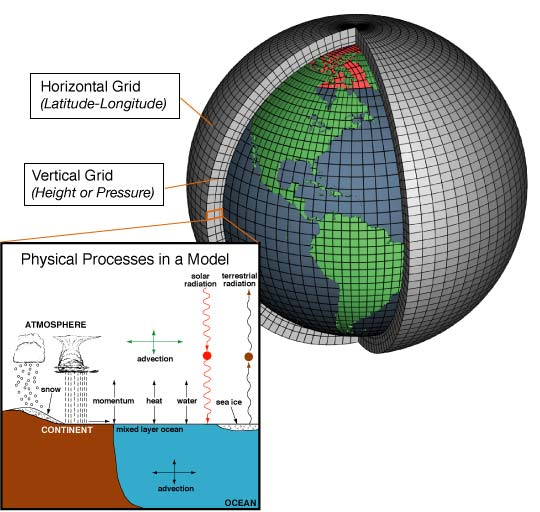
\includegraphics[width=1\linewidth]{../_chapter_materials/model_picture} \caption{Coupled global climate models simulate physical processes in both the atmosphere and from landscape/oceanic features (NOAA, public domain). Each cell in the climate model contains these features, and energy and matter may pass from one cell to another (the cells are not isolated).}\label{fig:model-fig}
\end{figure}

\begin{table}[t]

\caption{\label{tab:scenario-table}Characteristics of selected emissions scenarios from the Intergovernmental Panel on Climate Change. These scenarios represent alternative possibilities for future social and technological change as envisioned by a collaboration of governmental and non-governmental analysts.}
\centering
\resizebox{\linewidth}{!}{
\begin{tabular}{>{\raggedright\arraybackslash}p{20em}>{\raggedright\arraybackslash}p{10em}>{\raggedright\arraybackslash}p{10em}>{\raggedright\arraybackslash}p{10em}}
\toprule
Scenario.characteristics & A1B & A2 & B1\\
\midrule
\rowcolor{gray!6}  Human population growth & Low & High & Low\\
Globalization & High & Low & High\\
\rowcolor{gray!6}  Focus on environmental sustainability & Low & Low & High\\
Economic growth & Very high & Medium & High\\
\rowcolor{gray!6}  Land-use changes & Low & Medium/high & High\\
\addlinespace
Pace of technological developments (energy use) & Rapid & Slow & Medium\\
\rowcolor{gray!6}  Changes in energy use & Rapid; changes in both production and use & Slow; vary by region & Medium; shift to lowered use of materials\\
Realized energy use & Very high & High & Low\\
\bottomrule
\end{tabular}}
\end{table}

The community of climate change experts has developed different
storylines that describe alternative possible futures, which each has
its own projection of predicted quantities of GHG emissions (Table 1).
To predict the effects of GHG emissions on climate, scientists plug
predictions of GHG emissions into a CGCM to predict future climate under
different emissions scenarios.

\section{Objectives}\label{objectives}

You will work with output from a simulation run from the 3rd-generation
CGCM produced by the Canadian Center for Climate Modeling and Analysis.
This dataset focuses on near-surface air temperature - the same type of
temperature reported in the daily weather report. The temperature is
reported in mean temperature (\(^\circ\)K) for each month during the
21\textsuperscript{st}-century (2001-2100), giving a total of 1200
values for the 1200 consecutive months. You are provided these data for
the three emissions scenarios described in Table 1 (A1B, A2, B1) and a
fourth set of conditions representing ``Committed'' climate change. The
``Committed'' set of conditions assumes that the composition of the
atmosphere remains unchanged at year 2001 values (which has already been
proven entirely unrealistic). Therefore, the only climate changes that
will occur are those to which the climate system is already committed
due to changes in atmospheric concentration as of the year 2001. The
Committed scenario is not intended as a realistic scenario. Instead, it
serves as a pseudo control so that we can compare the other climate
scenarios to a baseline. By comparing the results of a given scenario
with the results under the Committed scenario, one can see how much
additional climate change a scenario produces compared to what would be
produced if alterations in climate forcing agents were arrested at 2001
levels.

Since climate is highly variable across the globe, you will focus on a
particular grid cell in a continuous North-South transect through North
America (Fig. 2) for questions 1 and 2. These grid cells will be
assigned either in lab, or on Canvas. For question 3, you will use all
of the data.

\begin{figure}
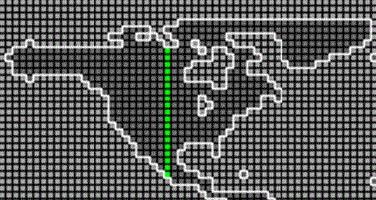
\includegraphics[width=5.22in]{../_chapter_materials/transect_picture} \caption{Location of latitudinal transect through North America for which you have data. The amount of sunlight reaching the earth's surface varies greatly along the transect (as does other seasonal features such as precipitation, ice-sheet cover, etc).}\label{fig:transect-fig}
\end{figure}

\pagebreak

\begin{enumerate}
\def\labelenumi{\arabic{enumi}.}
\tightlist
\item
  Will future near-surface air temperature be influenced by GHG
  emissions?

  \begin{itemize}
  \tightlist
  \item
    Seasonal variation in temperature will probably mask any long-term
    trends in temperature due solely to GHG concentrations. With that in
    mind, analyze data just using one month (July) in the dataset:

    \begin{itemize}
    \tightlist
    \item
      Make a graph {[}geom\_point(){]} showing how temperature in
      \textbf{July} varies across the 100 years of the simulation for
      all of the emissions scenarios.
    \end{itemize}
  \end{itemize}
\item
  Under the most extreme GHG emissions scenario (A2), will climate
  change have a greater effect in the winter or summer on near-surface
  temperatures?

  \begin{itemize}
  \tightlist
  \item
    Seasonal swings in irradiance is one of the primary natural
    control-knobs on temperature, so GHG emissions may cause temperature
    to change more in a particular season.

    \begin{itemize}
    \tightlist
    \item
      Repeat the prior analysis, but compare data from January and July
      (but only for the \textbf{A2 scenario}).
    \end{itemize}
  \end{itemize}
\item
  Under the most extreme GHG emissions scenario (A2), will climate
  change have a greater effect at high or low latitudes?

  \begin{itemize}
  \tightlist
  \item
    Irradiance is distributed unevenly across the globe, so the effect
    of GHG concentrations may differ based on location.

    \begin{itemize}
    \tightlist
    \item
      Create a graph examining 100-year mean temperature change (y-axis
      values) across latitude (x-axis values), which will help you
      address this question.
    \end{itemize}
  \end{itemize}
\end{enumerate}

Please provide statistical details when necessary (refer to your R
analysis file).

\pagebreak

\section{Lab report specifics}\label{lab-report-specifics}

\begin{enumerate}
\def\labelenumi{\arabic{enumi}.}
\tightlist
\item
  Introduction

  \begin{itemize}
  \tightlist
  \item
    How do GHGs influence climate?
  \item
    How do scientists study future climates?
  \item
    Objectives
  \item
    Hypotheses
  \end{itemize}
\item
  Methods

  \begin{itemize}
  \tightlist
  \item
    Model particulars and analysis steps
  \item
    Calculations / statistics
  \end{itemize}
\item
  Results

  \begin{itemize}
  \tightlist
  \item
    Question 1 (text \textbf{AND} graph)
  \item
    Question 2 (text \textbf{AND} graph)
  \item
    Question 3 (text \textbf{AND} graph)
  \end{itemize}
\item
  Discussion

  \begin{itemize}
  \tightlist
  \item
    Hypotheses rejected/supported
  \item
    Provide a coherent explanation/interpretation of your results
  \end{itemize}
\end{enumerate}




\newpage
\singlespacing 
\end{document}
